\documentclass[preprint, 3p,
authoryear]{elsarticle} %review=doublespace preprint=single 5p=2 column
%%% Begin My package additions %%%%%%%%%%%%%%%%%%%

\usepackage[hyphens]{url}

  \journal{An awesome journal} % Sets Journal name

\usepackage{graphicx}
%%%%%%%%%%%%%%%% end my additions to header

\usepackage[T1]{fontenc}
\usepackage{lmodern}
\usepackage{amssymb,amsmath}
% TODO: Currently lineno needs to be loaded after amsmath because of conflict
% https://github.com/latex-lineno/lineno/issues/5
\usepackage{lineno} % add
\usepackage{ifxetex,ifluatex}
\usepackage{fixltx2e} % provides \textsubscript
% use upquote if available, for straight quotes in verbatim environments
\IfFileExists{upquote.sty}{\usepackage{upquote}}{}
\ifnum 0\ifxetex 1\fi\ifluatex 1\fi=0 % if pdftex
  \usepackage[utf8]{inputenc}
\else % if luatex or xelatex
  \usepackage{fontspec}
  \ifxetex
    \usepackage{xltxtra,xunicode}
  \fi
  \defaultfontfeatures{Mapping=tex-text,Scale=MatchLowercase}
  \newcommand{\euro}{€}
\fi
% use microtype if available
\IfFileExists{microtype.sty}{\usepackage{microtype}}{}
\usepackage[]{natbib}
\bibliographystyle{plainnat}

\ifxetex
  \usepackage[setpagesize=false, % page size defined by xetex
              unicode=false, % unicode breaks when used with xetex
              xetex]{hyperref}
\else
  \usepackage[unicode=true]{hyperref}
\fi
\hypersetup{breaklinks=true,
            bookmarks=true,
            pdfauthor={},
            pdftitle={A view of the economic implications of AI as a potential General Purpose Technology},
            colorlinks=false,
            urlcolor=blue,
            linkcolor=magenta,
            pdfborder={0 0 0}}

\setcounter{secnumdepth}{5}
% Pandoc toggle for numbering sections (defaults to be off)


% tightlist command for lists without linebreak
\providecommand{\tightlist}{%
  \setlength{\itemsep}{0pt}\setlength{\parskip}{0pt}}







\begin{document}


\begin{frontmatter}

  \title{A view of the economic implications of AI as a potential
General Purpose Technology}
    \author[University of Helsinki]{Irina Vélez%
  \corref{cor1}%
  \fnref{1}}
   \ead{irina.velezlopez@helsinki.fi} 
    \author[Aalto University]{Otto Palkama%
  %
  \fnref{1}}
   \ead{otto.palkama@aalto.fi} 
      \cortext[cor1]{Corresponding author}
    \fntext[1]{Exchange Student.}
  
  \begin{abstract}
  This paper explores the potential of artificial intelligence (AI) and
  Language Models (LLMs) as general-purpose technologies (GPTs) that can
  drive growth and development. The generalization of tools,
  particularly in the realm of AI, enhances the potential for
  productivity improvements and opens up new possibilities for value
  creation. However, there can be a discrepancy between optimistic
  expectations and actual outcomes, which is a natural aspect of
  transformative periods. The paper discusses the coexistence of
  forward-looking optimism and backward-looking disappointment and
  emphasizes the time required for society to fully integrate and
  benefit from new technologies. It concludes by highlighting the
  importance of grounded expectations and the value of intangible assets
  in the process of economic transition.
  \end{abstract}
    \begin{keyword}
    General Purpose Technology \sep Artificial Intelligence \sep 
    Creative destruction
  \end{keyword}
  
 \end{frontmatter}

\hypertarget{introduction}{%
\section{1. Introduction}\label{introduction}}

The generalization of tools is a crucial factor in harnessing the
potential for growth and development. When a tool can be widely used for
various purposes, its value increases significantly. In the realm of
artificial intelligence (AI), Language Models (LLMs) serve as a
foundational technology for other tools, such as AI-powered software.
This opens up new possibilities and enhances the potential for
productivity improvements in the workforce. As mentioned by
\citep{gptaregpts}, LLMs like GPTs exhibit characteristics of
general-purpose technologies, which can have profound economic, social,
and policy implications.

The emergence of new capabilities and the widespread adoption of LLMs as
enablers of new AI-based tools, coupled with the increasing number of
users utilizing tools like ChatGPT, signifies a future that has not been
seen before. This accelerated expansion and pushing of boundaries and
limits hold the potential for transformative changes.

In light of these dynamics, it is important to recognize that while
there may be optimism surrounding new technologies, there can also be a
discrepancy between expectations and actual outcomes. This coexistence
of forward-looking optimism and backward-looking disappointment is a
natural aspect of periods of transformative change. It reflects the
human desire to witness the fulfillment of expectations within their
lifetime, while also acknowledging the time required for society to
fully integrate and benefit from these innovations.

\hypertarget{generalization-capabilities-of-llms-as-gpt}{%
\section{2. Generalization Capabilities of LLMs as
GPT}\label{generalization-capabilities-of-llms-as-gpt}}

Investigating the adoption rate of various GPTs, \citep{Chen2021HowDL}
examined how worker mobility affects the likelihood of an establishment
adopting a new general-purpose technolog{]}. By examining data from over
153,000 establishments between 2010 and 2018, it was observed how these
establishments made decisions regarding the adoption of machine
learning. The findings from the study showed a significant decline in
adoption likelihood when there were facilitations in worker movements.
According to the \citep{Helpman1996DiffusionOG}, both historical
evidence and theoretical models indicate that General Purpose
Technologies (GPTs), like the steam engine and electricity, are pivotal
for economic progress. The author further demonstrates that the stepwise
adoption of a GPT across sectors leads to a dual-phase cycle, ultimately
resulting in prolonged economic growth.

\hypertarget{key-factors-contributing-to-the-widespread-adoption-of-a-technology-as-a-gpt}{%
\subsection{Key factors contributing to the widespread adoption of a
technology as a
GPT}\label{key-factors-contributing-to-the-widespread-adoption-of-a-technology-as-a-gpt}}

General Purpose Technology is a transformative technology with a strong
improvement process at the begining and eventually becoming widely
adopted for its multiples uses, while producing many spillover effects
\citep{paradox}. As such, it have a pervasive impact on society as a
whole, mainly due to its capability to redefine the ways in which
businesses operate, improve productive and contribute to long-term
economic growth. Some well-know examples are steam power, electricity,
semiconductors, and internet.

The study by \citep{Qiu2018TheIG} observes a trend towards
internationalized innovation networks in multinational corporations.
Through a U.S. patent database from 1969-1995, it's found that the
development of general purpose technologies (GPTs) is tied to the
globalization of corporate innovations. The observations are in line
with \citep{Chen2021HowDL}, which further finds that actors such as
establishment characteristics and industry conditions play a crucial
role in this adaptation. Notably, establishments with greater size, more
large establishments in their vicinity, and heightened experimentation
with analytics technology exhibit a particularly healthy environment for
the widespread adoption of a technology as a GPT.

Until now the abilities reached by the Large Languages Models LLMs have
arisen to a certain level of computational power that might require
scaling up past this threshold (10\^{}23 training FLOPs), meaning that
they are able to perform multiple tasks related to Text Understanding
and Generation,Problem Solving and Mathematics, Image and Data
Classification, Text Analysis and Comprehension, and so on, but as
\citep{weiemergent} suggested for future works, it could be possible new
abilities could emerge scaling up the models and understanding how
emergence occurs would provide new insights into how to train
more-capable language models. The emergence of these skills are one of
the key factors of becoming in a GPT.

Artificial intelligence a term coined by emeritus Stanford Professor
John McCarthy in 1955, was defined by him as ``the science and
engineering of making intelligent machines''.\footnote{Available at:
  https://hai.stanford.edu/sites/default/files/2020-09/AI-Definitions-HAI.pdf}
These systems are designed to simulate human cognitive abilities, such
as learning, reasoning, problem-solving, perception, and language
understanding. Within the realm of AI, Large Language Models (LLMs) are
a specific type of AI model that utilizes deep learning techniques,
particularly neural networks, to process and generate human-like
language. LLMs are trained on vast amounts of text data and can perform
tasks like language translation, text summarization, and question
answering.

In the past, computer programs were developed by painstakingly encoding
human knowledge, following a precise set of instructions that mapped
specific inputs to desired outputs. This approach required programmers
to meticulously define every step of the process. However, machine
learning systems operate differently. They utilize general algorithms,
such as neural networks, which enable them to independently determine
the appropriate mapping between inputs and outputs. This is achieved
through exposure to extensive datasets containing numerous examples. By
analyzing and learning from these examples, machine learning systems can
identify patterns and make accurate predictions or classifications
without explicit programming instructions.

\hypertarget{what-is-the-potential-economic-impact-of-ai}{%
\section{3. What is the potential economic impact of
AI?}\label{what-is-the-potential-economic-impact-of-ai}}

Considering the potential of AI as a new GPT, assessing its possible
contribution to economic growth is worthwhile in times of dizzying
change such as the present. The winds of uncertainty are blowing
everywhere and it would be useful to set expectations. Given the
conditions of uncertainty and the low accuracy of predictions, the
assessment of its potential impact seems to be addressed only by a
retrospective approach, which means that the performance of previous
general-purpose technologies, such as steam power, electricity or the
Internet, could provide a more realistic answer to this question.

However, this topic has already been addressed by \citep{paradox} and
\citep{Nicholas}, in a context where there are optimists and pessimists
about technology and growth. A real dichotomy emerges between the higher
profit expectations of forward-looking entrepreneurs and the poor growth
performance reflected in retrospective statistics.

One example mentioned by \citep{paradox} is the call center industry,
which had approximately 2.2 million agents in 2015 in the United States.
It was plausible at that time to anticipate that voice recognition
systems like IBM's Watson could potentially reduce the number of workers
by 60\%. However, in hindsight, it is evident that the expectations have
not been fully met, as shown in Figure \ref{fig1}, which illustrates the
statistics.

\begin{figure}

{\centering 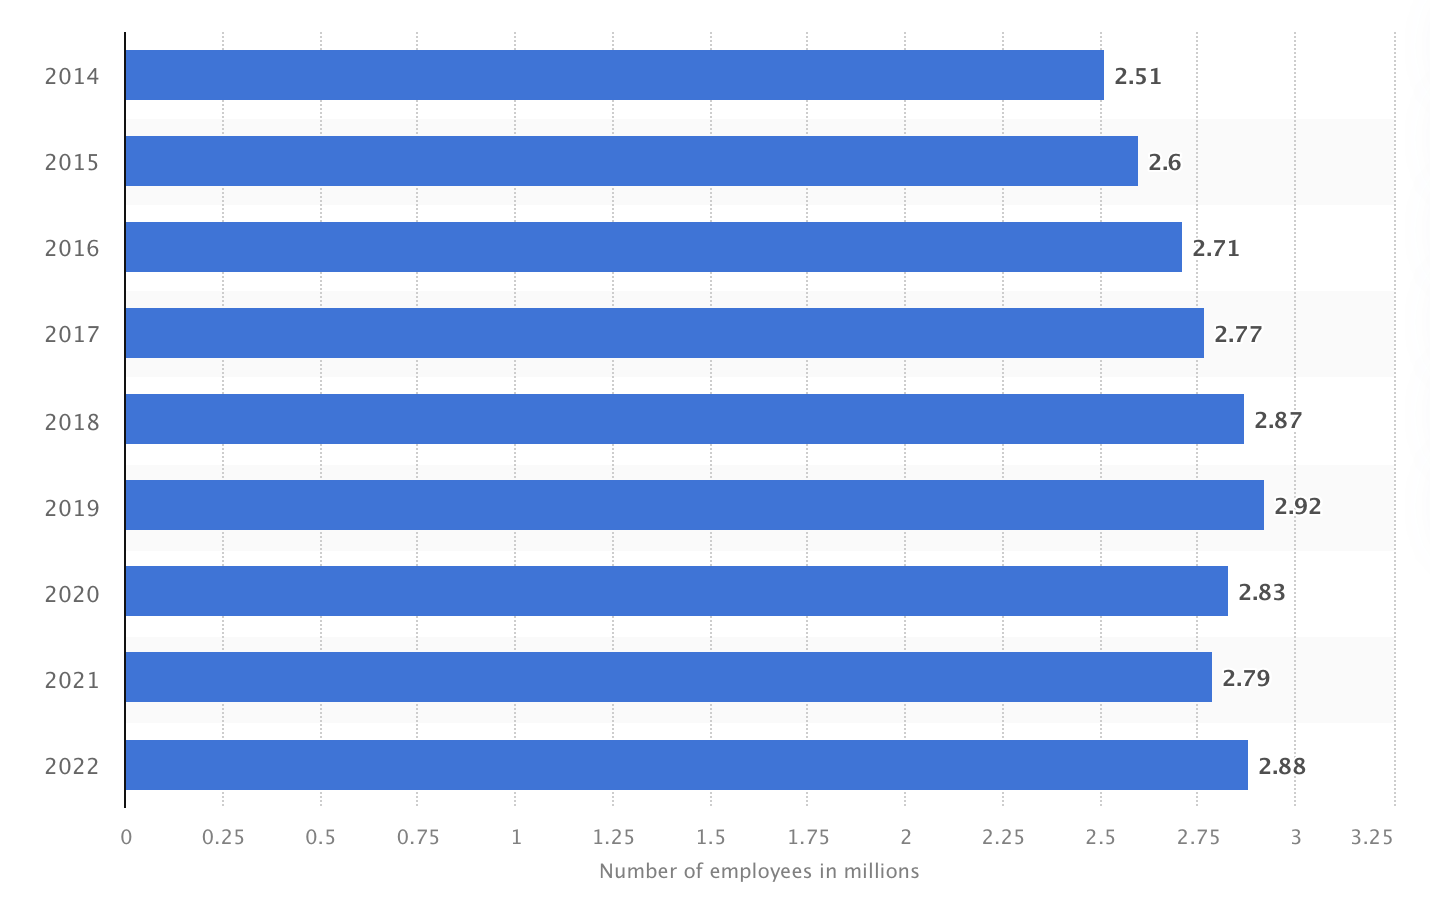
\includegraphics[width=0.7\linewidth]{../Views/contact_center_employees_US} 

}

\caption{\label{fig1}Number on contact center employees in the United States from 2014 to 2022.}\label{fig:fig1}
\end{figure}

As \citep{paradox} explains, this apparent incongruity is due to the
time lag between the creation of the technology and the full realization
of its benefits in the economy and society. It takes time to build up
the stock of the new technology, develop the necessary human capital
skill set, undergo the process of re-engineering business process
transformations, and develop complementary innovations for full
realization in the real economy.

To support this explanation of the lag, the Schumpeterian growth model
could offer another good perspective, taking as a starting point that
the real contributions to growth are value creation and cost
optimization, so AI should be at the service of these contributors to
growth.

\hypertarget{assessing-the-potential-economic-impact-of-ai-in-terms-of-value-creation-and-cost-optimization.}{%
\subsection{Assessing the potential economic impact of AI in terms of
value creation and cost
optimization.}\label{assessing-the-potential-economic-impact-of-ai-in-terms-of-value-creation-and-cost-optimization.}}

From an economic perspective, one of the fundamental problems in
understanding corporate behavior is the pursuit of profit maximization
by firms. This objective drives economic growth and leads to two main
objectives in the private business sector: adjusting the production
function to obtain the right quantities to supply the market, while
coping with constraints, often in the form of a limited budget.

The firm's goal of maximizing profits can be represented as follows: \[
Profit = Total \ Income - Total \ Costs: \Pi = PX - C(X)
\] \[
Maximization \ Problem: \max_{x} \Pi(X) = PX - (wL + rK)
\]

Where PX represents the revenue generated by production function X, and
C(X) represents the corresponding costs associated with labor and
capital costs. Thus, on one side of the coin, value creation contributes
to increasing profits by adjusting the output of production function X,
while on the other side, cost optimization aims to mitigate not only
budget constraints but also resource constraints. Therefore, AI must be
oriented towards achieving one or both of these objectives to promote
growth.

To exemplify value creation through AI, consider the use of deep neural
network systems in skin cancer diagnosis \citep{cancer}, fraud detection
and risk assessment in the financial sector, and inventory forecasting
automation, as seen in Amazon's AI-powered inventory management product.
On the other hand, from a cost optimization perspective, AI is used in
predictive maintenance and quality control to anticipate equipment
failures\footnote{Available at:
  https://www.ge.com/research/project/predictive-maintenance}.

\hypertarget{shumpenters-concept-of-creative-destruction}{%
\subsection{Shumpenter's concept of creative
destruction}\label{shumpenters-concept-of-creative-destruction}}

Creative destruction refers to the process of creating and developing
new technology that continuously disrupt and replace the existing
obsolete technology in order to drive economic progress and
growth.\footnote{Definition created with the help of
  \href{https://github.com/mukulpatnaik/researchgpt.git}{ResearchGPT}}.

Thus, let us consider two types of companies, those that are creators of
new technologies and major investors in R\&D, such as the big technology
companies like Apple, Amazon, Meta or Google, called ``creators'' of
technology, and on the other hand, companies that adopt and implement
the new technology in order to maximize their profits through the
greater added value created by their production functions and cost
optimization, or both, called ``adopters'' of technology.

Knowledge or innovation is considered a \textbf{public good}, one you
have invented something , it is almost free to spread it around the
world. Thus, the first initial cost of producing the technology has to
be covered through monopoly profits (Creators), because this has been
the mechanism that the market system has found to cover the huge initial
costs\footnote{Insights taken from this
  \href{https://youtu.be/m3nkTrFF2zs?si=dgPJlvVgQuuQAcL8}{Bilkent
  Üniversitesi lecture}}.

Once the new technology has been widely launched in the market at an
almost affordable or even free price, as in the case of ChatGPT, the
maturity level or readiness of the adopter must be high in order to take
advantage of the full potential of the new technology. From the
adopter's point of view, it takes time to evolve and incorporate the new
technology into their business process in a way that is effective and
beneficial to the business. This evolution requires developing new
business processes, adjusting their production functions to add value to
their bottom line, and reallocating skilled human capital to address the
transformation.

Destruction is represented in the Schumpeterian Growth Model as the
expected years that firms will remain in the market, if they do not
adapt. And this adaptation process is mainly promoted by the creation of
new ideas E{[}A{]}. This time expectation is represented by the
following equation

\[
Firm \ Lifetime: E[\tau] = 1/E[A]
\] \[
Firm \ Lifetime: E[\tau] = 1/\gamma N
\] Where: New ideas corresponds to \(E[A] = \gamma N\)

The life of the company is reduced by the increase in productivity
(\(\gamma\)) and the deployment of new technologies (N). This leads to
two transition scenarios

\begin{enumerate}
\def\labelenumi{\arabic{enumi}.}
\item
  If the adopter is not able to incorporate the new technologies or take
  advantage of them, its profit will be decreasing until a possible exit
  from the market, when its profits will be zero, and therefore, this
  company will not contribute to the growth of the economy.
\item
  If the adopting company is able to incorporate the new technology or
  take advantage of it, its profit will increase, which in turn will
  ensure its permanence in the market. However, this benefit is not
  immediately reflected in the aggregate accounting statistics. The
  adaptation process takes time, due to the development of new business
  processes, to the improvement of the qualification of its human
  capital, to the time required for the reallocation of more qualified
  human capital from less capable companies to companies with more
  potential for growth or success.
\end{enumerate}

This reallocation of human capital can be seen in one of the key
statistics in the labor market: Job postings.The number of AI related
job postings has increased on average from 1.7\% in 2021 to 1.9\% in
2022 according to \citep{reportAI}. This increased trend can be seen in
Figure \ref{fig2}. In 2022, the top three countries with the higher
percentage of AI job postings were the United States (2.1\%), Canada
(1.5\%), and Spain (1.3\%).

\begin{figure}

{\centering 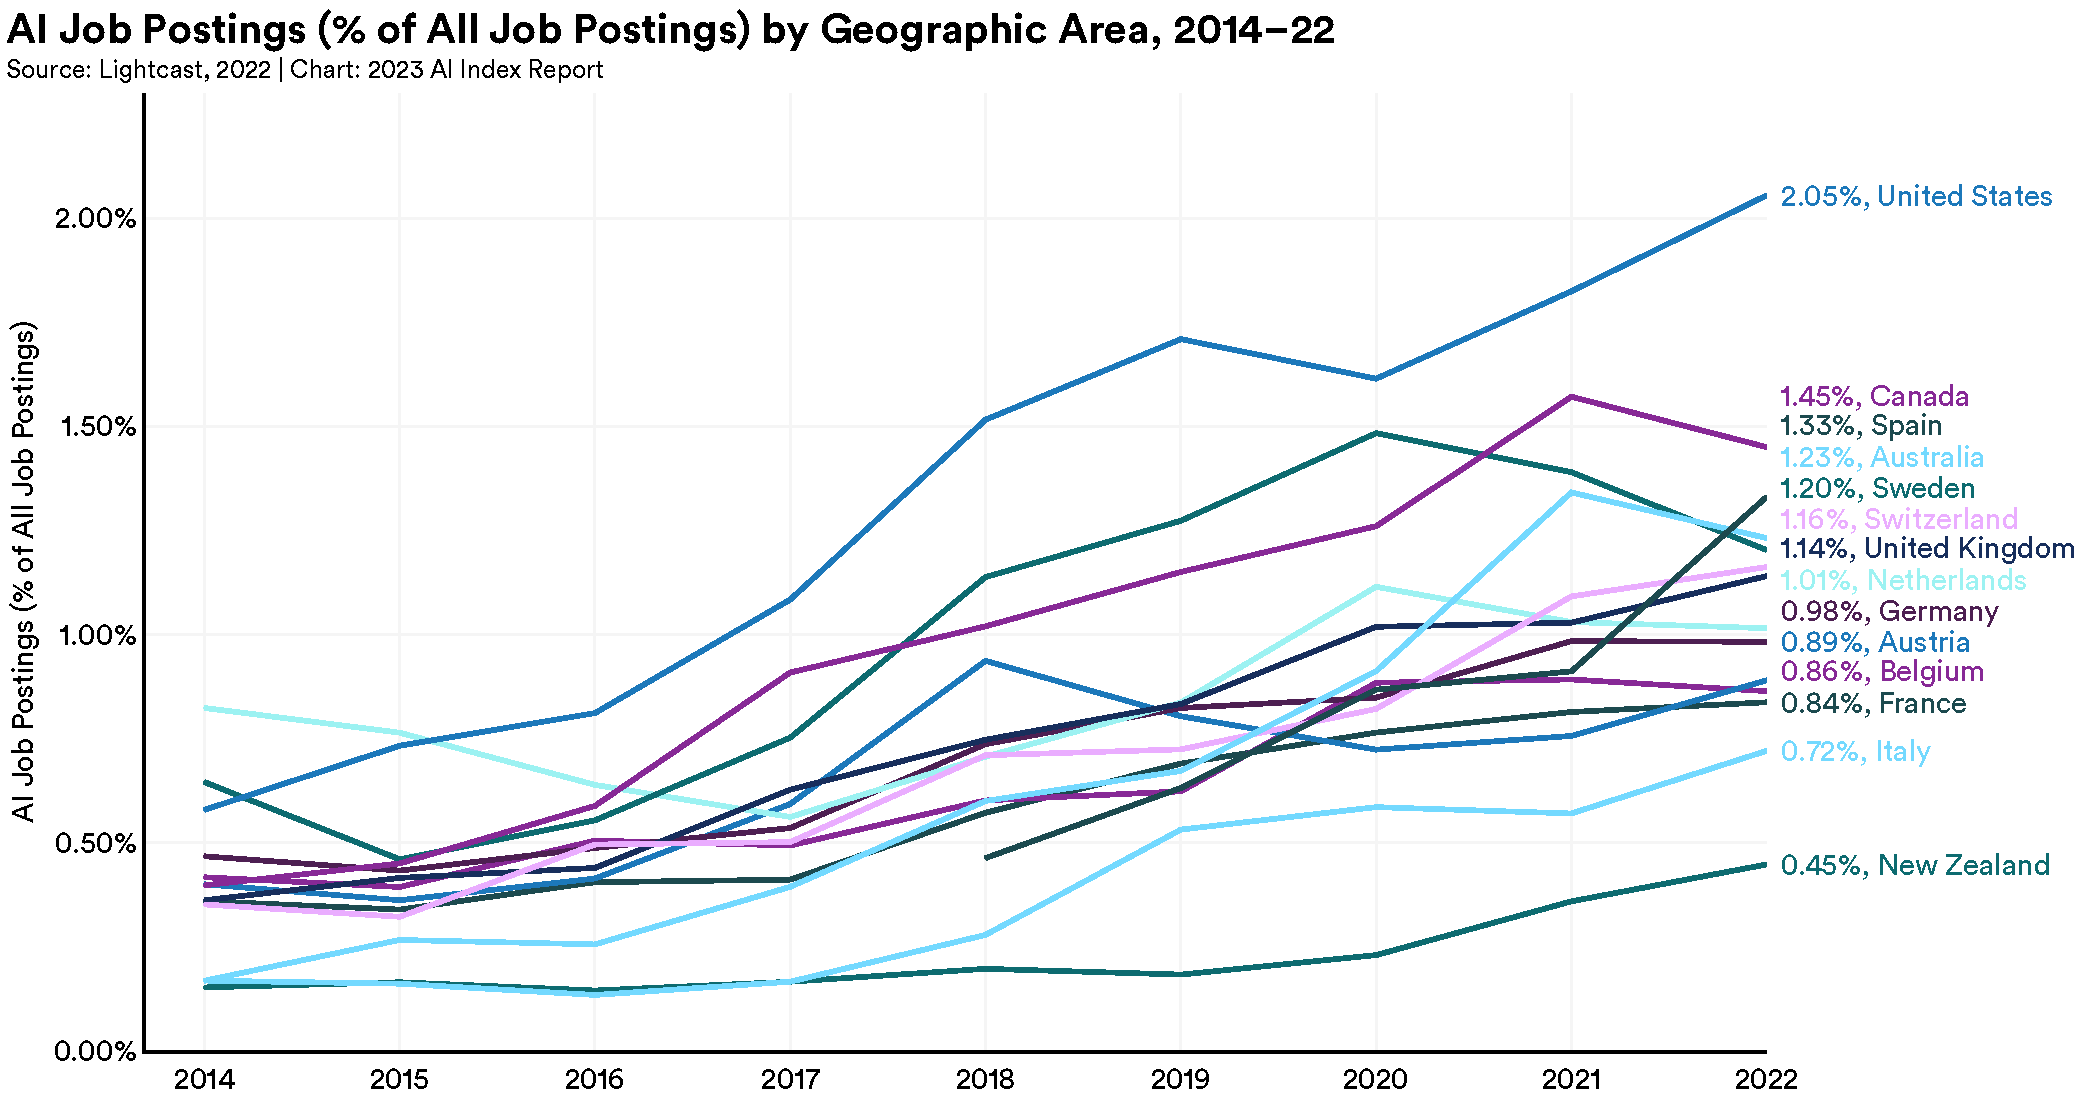
\includegraphics[width=0.7\linewidth]{../Views/AI_job_postings_by_geo_area} 

}

\caption{\label{fig2} Percentage of all job postings that require some kind of AI skill by Geographic Area, 2014 to 2022.}\label{fig:fig2}
\end{figure}

Thus, in times of structural change such as the present, it is difficult
to see the results of these new technologies, as the contributions to
growth that successful firms might make are offset by the declining
profits of outgoing firms. Therefore, it is reasonable to think that the
statistics do not yet reflect the potential benefits of using AI.

This can be illustrated by reviewing the investments in AI over the last
decade and the historical behavior of the Multiple Factor of
Productivity. Figure \ref{fig3} shows an upward trend in global AI
investments over the last decade, with the exception of 2022, when, for
the first time since 2013, global business investment in AI has
declined.

\begin{figure}

{\centering 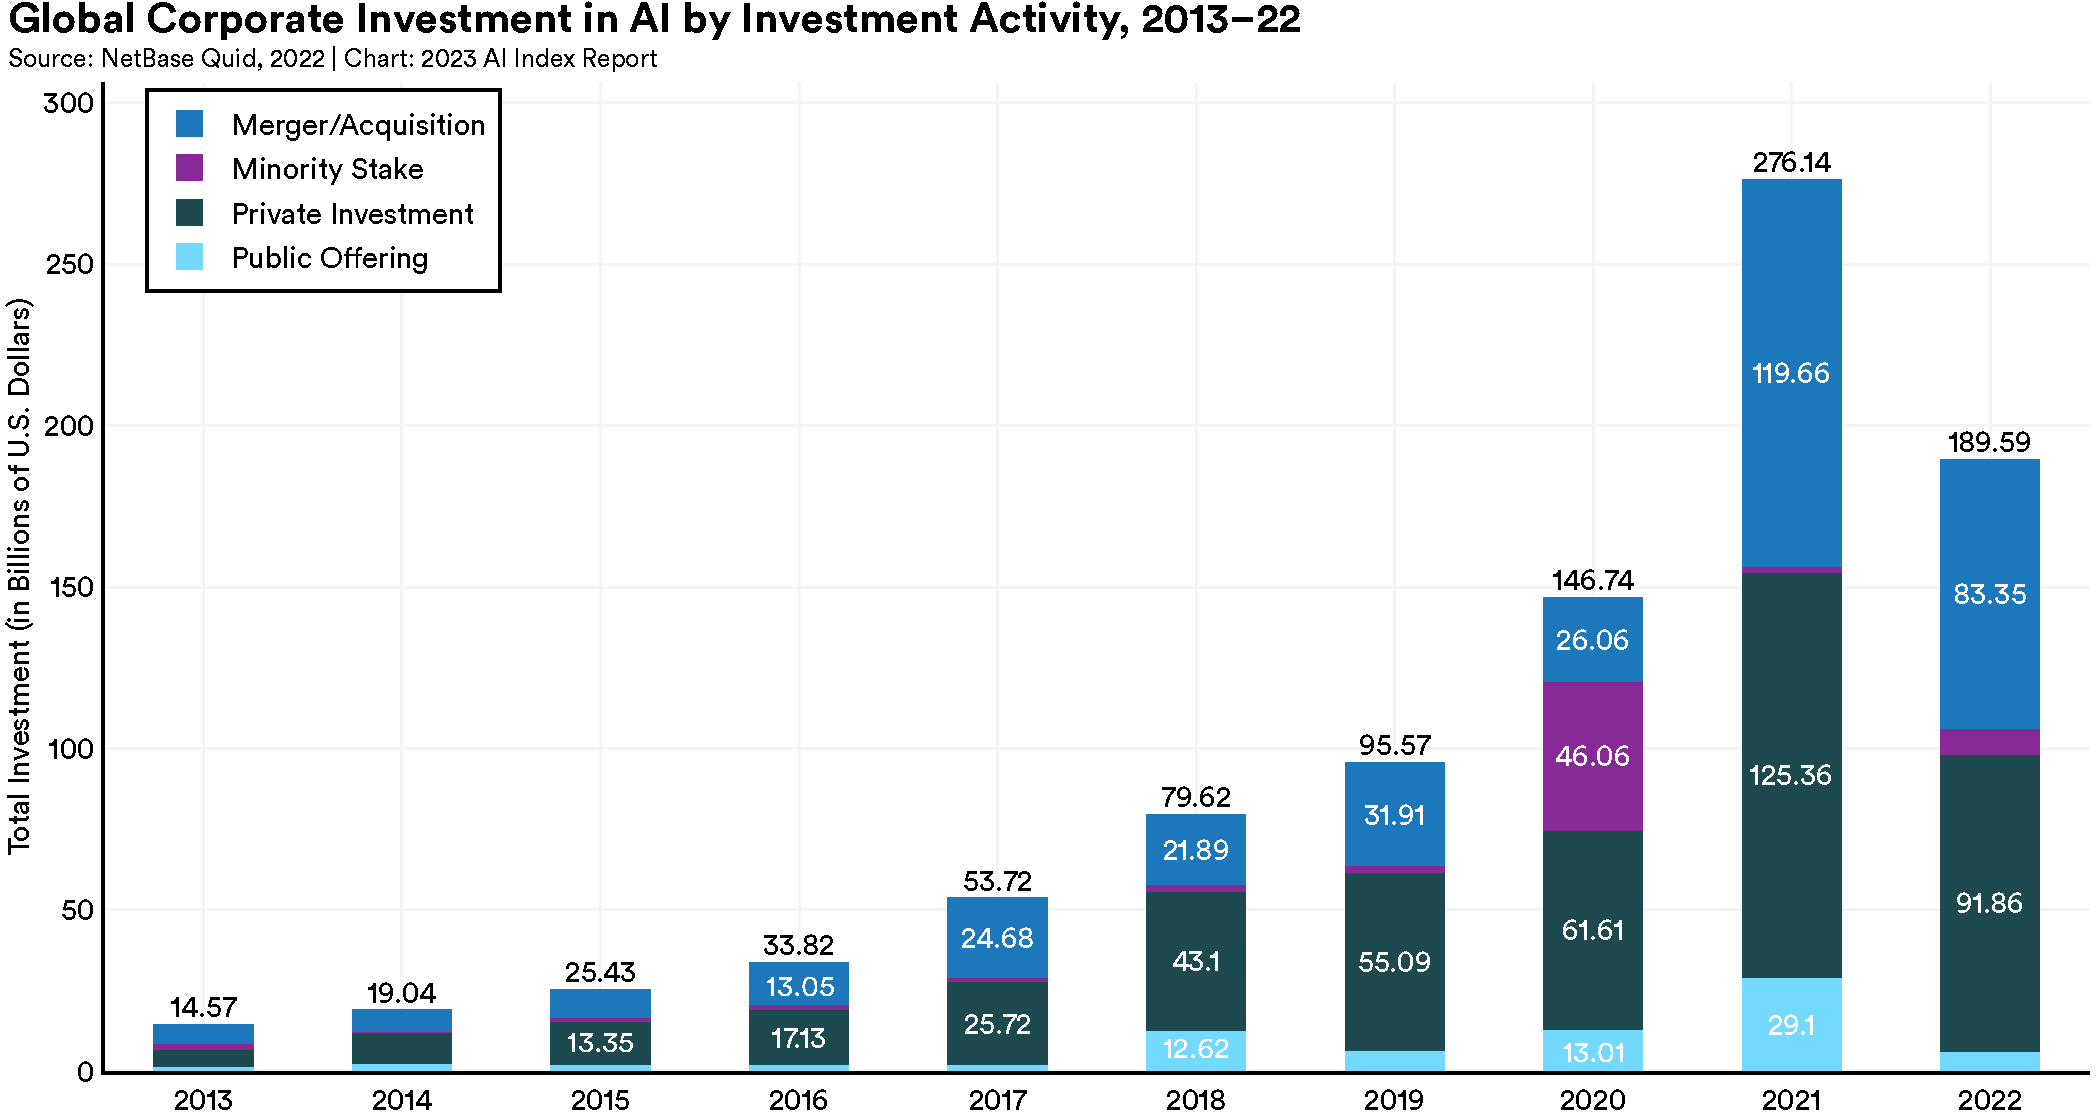
\includegraphics[width=0.7\linewidth]{../Views/global_investiment_by_inv_activity} 

}

\caption{\label{fig3}Global Corporate Investment in AI by Investment Activity, 2013 to 2022.}\label{fig:fig3}
\end{figure}

However, these investments are not yet paying off in increases in the
productivity multiple factor, as can be seen in Figure 4 and Figure 5.

\begin{verbatim}
## 
## Attaching package: 'dplyr'
\end{verbatim}

\begin{verbatim}
## The following objects are masked from 'package:stats':
## 
##     filter, lag
\end{verbatim}

\begin{verbatim}
## The following objects are masked from 'package:base':
## 
##     intersect, setdiff, setequal, union
\end{verbatim}

\begin{figure}

{\centering 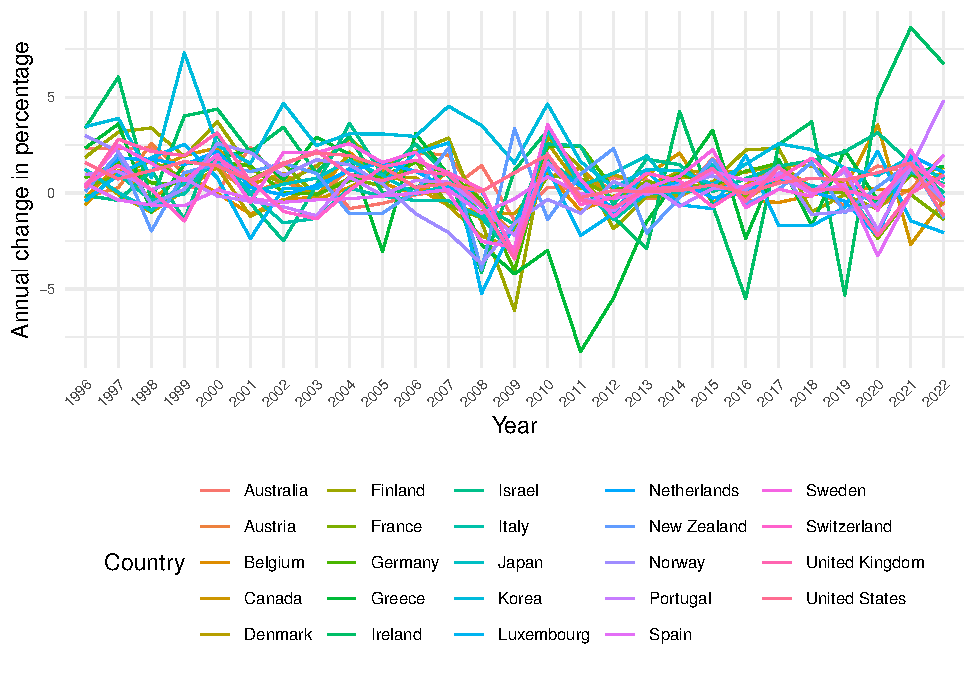
\includegraphics{Document_files/figure-latex/fig4-1} 

}

\caption{\label{fig4}Annual change of Multi Factor Productivity by OECD Country, 1996 to 2022.}\label{fig:fig4}
\end{figure}

Figure \ref{fig5} shows a decreasing trend in multifactor productivity
since 1996, but this trend has not changed despite investments in AI
since 2013. Therefore, this is an indicator that new technologies such
as AI has not yet reflected its benefits in the economy.

\begin{verbatim}
## `geom_smooth()` using formula = 'y ~ x'
\end{verbatim}

\begin{figure}

{\centering 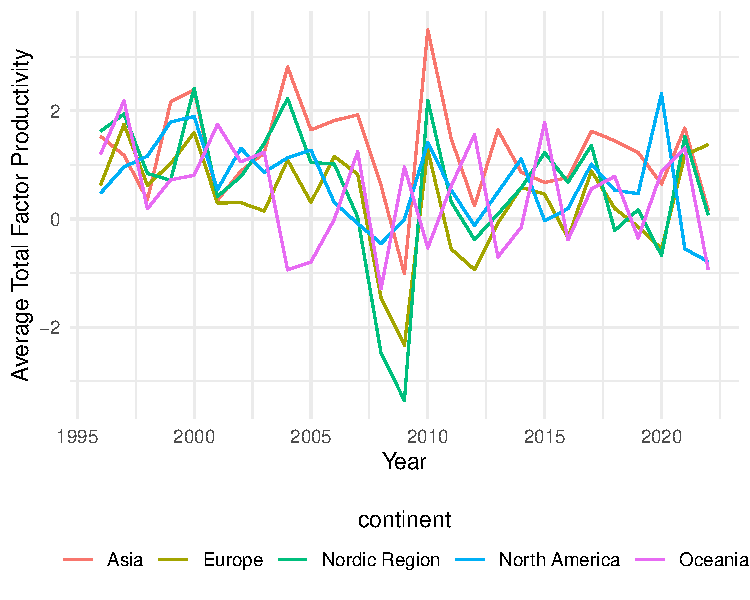
\includegraphics{Document_files/figure-latex/fig5-1} 

}

\caption{\label{fig5}Mean and median of Multifactor Productivity by year, 1996 to 2022. The dashed black lines represent the mean and median trend line}\label{fig:fig5}
\end{figure}

However, this result may not be entirely accurate, as the measurement
tools available to us today may not be capturing the real impact of
these technologies. Mainly because multifactor productivity growth is
measured as a residual, i.e., the part of GDP growth that cannot be
explained by growth in labor and capital inputs. Traditionally, TFP
growth has been considered to reflect technological progress, but in
practice this does not mean that this parameter reflects all the
benefits.

To exemplify this, let's think that a country with an amount R of
resources can allocate part of them (Creators) to do R\&D, while others
(Adopters) to produce a certain level of activity or result X.

Creators: Proportion n does R\&D: \(nR\). Adopters: The remainder goes
to produce X: \((1-n)R\).

If we think of these companies as a composite of human capital, creators
are individuals with the necessary skills to create new technologies,
while adopters are individuals with sufficient skills to produce X in
the traditional business model. Now, adopters need to acquire new skills
in order to incorporate the benefits of technology, creating new
business processes and successfully transitioning their production from
the old schemes to the new schemes. These adopters are investing in
intangible assets that the metrics are not reflecting. More importantly,
adopters need the help of creators to facilitate the adoption process in
their industries, because it stands to reason that creators are the most
skilled human capital part of the available resources.

This similar approach of dividing efforts into doing R\&D and producing
the product should be adopted by adapting firms, in the sense that those
doing R\&D are actually the ones leading the company's successful
transition to a new business model. In practical terms, from the
perspective of an adopting company:

Business Transformers: The ratio n avoids exiting the market: \(nR\).
Change assimilators: This ratio continues to maximize profit in the new
business model: \((1-n)R\).

Since consumers are not part of the production process, they have been
left out of this analysis. However, their acceptance towards the
consumption of AI-based products and their expected increase in the
consumption of AI-based services will have a positive impact on economic
growth.

Thus, the intangible assets associated with the transformation process
are not yet quantified and in the last wave of computerization their
value was about ten times greater than the direct investments in the
computer hardware itself \citep{paradox}. Thus, it is plausible that the
intangibles associated with AI are of comparable or greater magnitude.

\hypertarget{llms-vs.-artificial-general-intelligence-agi}{%
\section{4. LLMs vs.~Artificial General Intelligence
(AGI)}\label{llms-vs.-artificial-general-intelligence-agi}}

\hypertarget{understanding-the-difference-between-llms-and-agi}{%
\subsection{Understanding the difference between LLMs and
AGI}\label{understanding-the-difference-between-llms-and-agi}}

Large Language Models (LLMs) and Artificial General Intelligence (AGI),
represent distinct approaches to AI. Understanding their differences and
how they link together is crucial in navigating the evolving landscape
of AI research and applications. AGI, as defined by
\citep{Zhou2023PathTM} is a highly autonomous entity with the remarkable
capacity to comprehend, learn, and apply knowledge across an extensive
array of tasks and domains. Unlike narrow AI systems, AGI aims to
replicate the breadth of human cognitive abilities. This ambition makes
AGI the pinnacle objective within the field of artificial intelligence.
One of the key distinctions between LLMs and AGI lies in their scope of
intelligence. LLMs are specialized, focusing solely on language-related
tasks. Another critical difference is in learning and adaptation. AGI
systems, are designed for continual learning and adaptation. As
described by \citep{Wang2012Chapter1I} AGI's ability to be generalized
on fundamentally new areas.

\hypertarget{exploring-whether-agi-is-the-real-general-purpose-technology}{%
\subsection{Exploring whether AGI is the real General Purpose
Technology}\label{exploring-whether-agi-is-the-real-general-purpose-technology}}

The question of whether AGI can be considered the real General Purpose
Technology is soon to become more relevant, as AGI has not yet reached
its full potential and audience. While advanced LLM models like OpenAI's
ChatGPT have undoubtedly revolutionized the way people work in a wide
range of tasks, they represent just a glimpse of what AGI could
ultimately achieve. AGI, with its aspiration to replicate human-like
general intelligence across various domains, holds the promise of
transcending the limitations of narrow AI and becoming the ultimate tool
for problem-solving and innovation. Paper by
\citep{Mikki2023ArtificialGI} introduces the intriguing idea that
achieving AGI may necessitate noncomputable systems. This concept
challenges conventional thinking in AI by encouraging us to expand our
understanding of AGI's potential. It suggests that AGI might require
unconventional approaches beyond traditional computational frameworks.
While AGI has not yet fully realized its capabilities, it holds the
promise of reshaping the technological landscape. Mikki's proposal of
noncomputable systems, when integrated with other development ideas,
offers a tantalizing glimpse into the future of AGI, where its
transformative power knows no bounds.

\hypertarget{acknowledging-benefits-and-limitations-of-llms-as-gpt}{%
\section{5. Acknowledging Benefits and Limitations of LLMs as
GPT}\label{acknowledging-benefits-and-limitations-of-llms-as-gpt}}

\hypertarget{discussing-the-potential-benefits-of-llms-as-gpt}{%
\subsection{Discussing the potential benefits of LLMs as
GPT}\label{discussing-the-potential-benefits-of-llms-as-gpt}}

One of the significant advantages of incorporating LLMs as GPT is the
potential for substantial productivity gains. LLMs excel in natural
language understanding and generation, making them valuable tools for
automating tasks that involve processing and generating text. From
content generation to customer support automation, LLMs can streamline
processes, reduce labor costs, and boost efficiency. By automating
routine language-related tasks, they free up human resources to focus on
more creative and complex endeavors. In fields such as finance,
healthcare, and market analysis, LLMs can assist in extracting valuable
insights from unstructured data, leading to better-informed decisions
and strategies.

\hypertarget{addressing-the-limitations-and-challenges-associated-with-llms-as-gpt}{%
\subsection{Addressing the limitations and challenges associated with
LLMs as
GPT}\label{addressing-the-limitations-and-challenges-associated-with-llms-as-gpt}}

While LLMs offer significant potential as GPT, it is essential to
acknowledge the limitations and challenges associated with their
widespread adoption. The use of LLMs raises ethical concerns,
particularly in content generation and manipulation. LLMs rely on large
datasets for training, often containing sensitive information.
Safeguarding data privacy and ensuring compliance with data protection
regulations is an ongoing challenge that must be addressed to harness
the full potential of LLMs.

\hypertarget{conclusion}{%
\section{6. Conclusion}\label{conclusion}}

Positive expectations around new technologies that drive development,
economic growth and profit generation are often accompanied by optimism
on the part of industry leaders, technology experts and venture
capitalists. This optimism leads to speculative investments and
forecasts of future corporate wealth in the financial sector. However,
as \citep{paradox} suggests, there is no inherent contradiction between
forward-looking technology optimism and backward-looking disappointment.
The two can coexist, especially in periods of transformational change.
This can be attributed to human nature, as individuals want to see their
expectations fulfilled during their lifetime. However, it takes time for
society to fully incorporate and benefit from new technologies,
resulting in a slower rate of assimilation.

Although we are not concluding anything new to what has been mentioned
before by several authors, it has been worthwhile to review especially
the position of \citep{paradox} from the vision of the Schumpeterian
growth model, and some metrics such as the Multifactor productivity and
investments in AI, which allow us to have more grounded expectations of
these new technologies, without ignoring the value of the intangible
assets that are part of this process of economic transition.

\renewcommand\refname{References}
\bibliography{mybibfile.bib}


\end{document}
